\documentclass[../main.tex]{subfiles}
\begin{document}

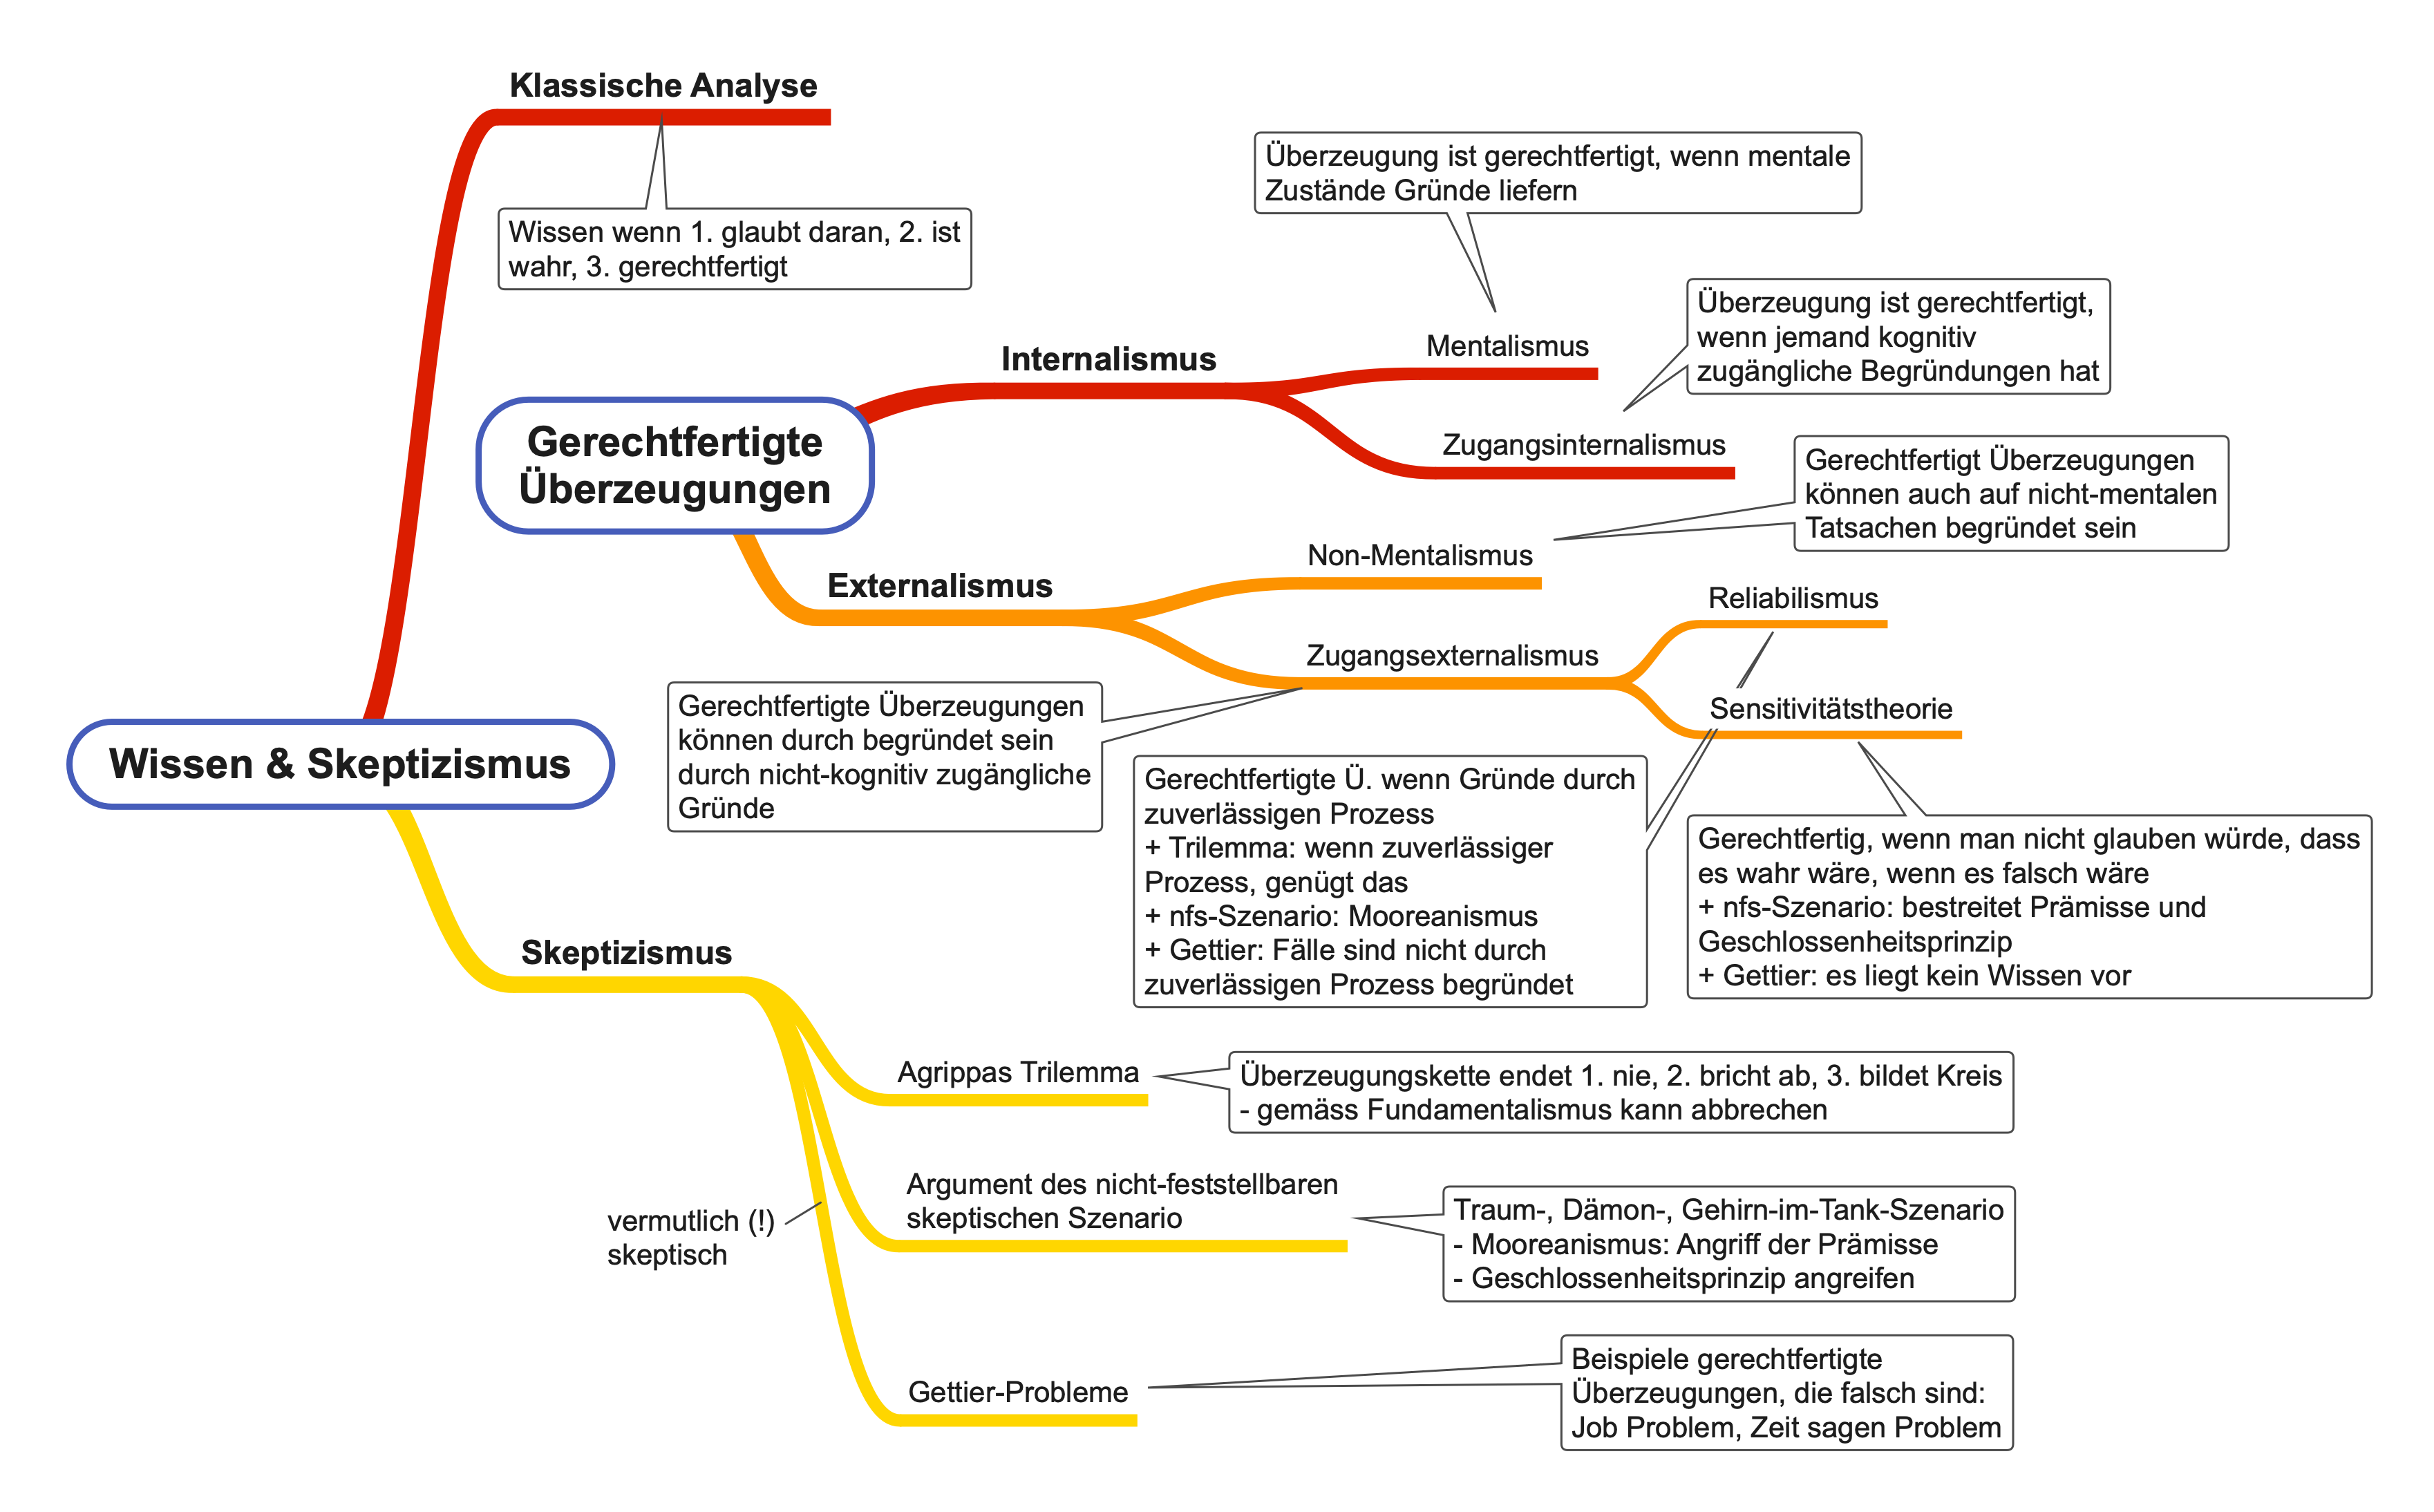
\includegraphics[width=\textwidth]{images/Wissen_und_Skeptizismus_Uebersicht.png}

\section{Arten des Wissens}
\begin{enumerate}
	\item Wissen von Tatsachen, auch \textit{Wissen-dass} (propositionales Wissen) wie z.B. <<Ich weiss, dass Paris in Frankreich ist.>>
	\item Wissen durch Bekanntschaft wie z.B. <<Ich kenne Paris.>>
	\item Praktisches Wissen/Fähigkeiten (prozedurales Wissen) wie z.B. <<Ich kann schwimmen.>>
\end{enumerate}

\section{Analyse des Wissens}
Die Frage nach Wissen begründet sich in den (1) notwendigen und (2) hinreichenden Bedingungen für Wissen. Anders: Welche Eigenschaften muss Wissen mindestens erfüllen? 
\subsection{Klassische Analyse von Wissen}
\paragraph{These} Folgende Bedingungen sind im Gesamten hinreichend (einzeln notwendig), damit man von Wissen (= gerechtfertigte Überzeugung) reden kann:
\begin{enumerate}
	\item Eine Person \textit{glaubt} an die Wahrheit des Sachverhalts
	\item Der Sachverhalt ist \textit{objektiv wahr}.
	\item Der Glaube an die Wahrheit des Sachverhalts ist durch die Person \textit{gerechtfertigt / gut begründet}
\end{enumerate}

\section{Skeptizismus}
\subsection{Was ist Skeptizismus} 
Der Skeptizismuswurde von Pyrrhon von Elis (4./3. Jh. v. Chr.) begründet und danach in der akademischen Skepsis von Akesilaos und Karneades weitergeführt. Heute gilt er als \textit{hypothetische} Gegenposition.

\subsubsection{Arten des Skeptizismus}
\begin{itemize}
	\item \textbf{Lokaler Skeptizismus} leugnet, dass wir Wissen in Bezug auf einen besonderen Typ von Tatsachen haben können. So zum Beispiel im Fall, dass wir kein Wissen über Zustände anderer oder dass wir wir kein Wissen über die Aussenwelt haben können. 
	\item \textbf{Allgemeiner (globaler) Skeptizismus} bezeichnet die Haltung, dass wir \textit{überhaupt kein Wissen} haben können, also dass Wissen unmöglich ist. 
\end{itemize}

\subsection{Skeptische Argumente}
Als skeptische Argumente bezeichnen wir Argumente des \textit{globalen} oder \textit{lokalen} Skeptizismus, deren Schlussfolgerung immer im Fazit endet, dass wir keine auf eine Art kein Wissen haben können. Sie sind sozusagen eine Sackgasse der Argumentation. 

Diese Sackgasse ist nicht zu verwechseln mit der kritischen Haltung gegenüber Argumenten und Behauptungen. Denn das Ziel der skeptischen Analyse, vor allem bezogen auf die klassische Analyse des Wissens, ist, dass Punkt 3. (unsere Überzeugungen müssen begründet sein) nie erfüllt werden kann und wir deswegen nie gegen alle Vorwürfe erhabenes Wissen haben können. 

\subsubsection{Agrippas Trilemma (Münchhausen-Trilemma)}
Dem unbekannten Skeptiker Agrippa zugeschrieben, besagt das Trilemma, dass eine Überzeugung immer durch andere Überzeugungen gerechtfertig wird, die wiederum durch andere Überzeugungen gerechtfertig werden muss. Die entstehende \textit{Rechtfertigungskette} endet 
\begin{enumerate}
	\item nie: sie ist unendlich (unendlicher Regress) oder 
	\item an einem Punkt (bricht ab): Dogmatismus oder
	\item am Anfang, bildet also einen Kreis (Zirkularität).
\end{enumerate}
Für keinen dieser Fälle lässt sich sagen, dass unsere Überzeugung gerechtfertig ist. Gerechtfertigte Überzeugungen (und damit Wissen) sind also per se nicht möglich. 
\paragraph{Einwände}
\begin{enumerate}
	\item Der \textbf{Fundamentalismus} besagt, dass eine Rechtfertigungskette unter bestimmten Umständen unproblematisch abbrechen kann. Es ist also falsch, dass eine Überzeugung notwendigerweise von anderen Überzeugungen gestützt werden muss. Dies nennt man \textbf{nicht-inferentielle Rechtfertigung}
\end{enumerate}

{\centering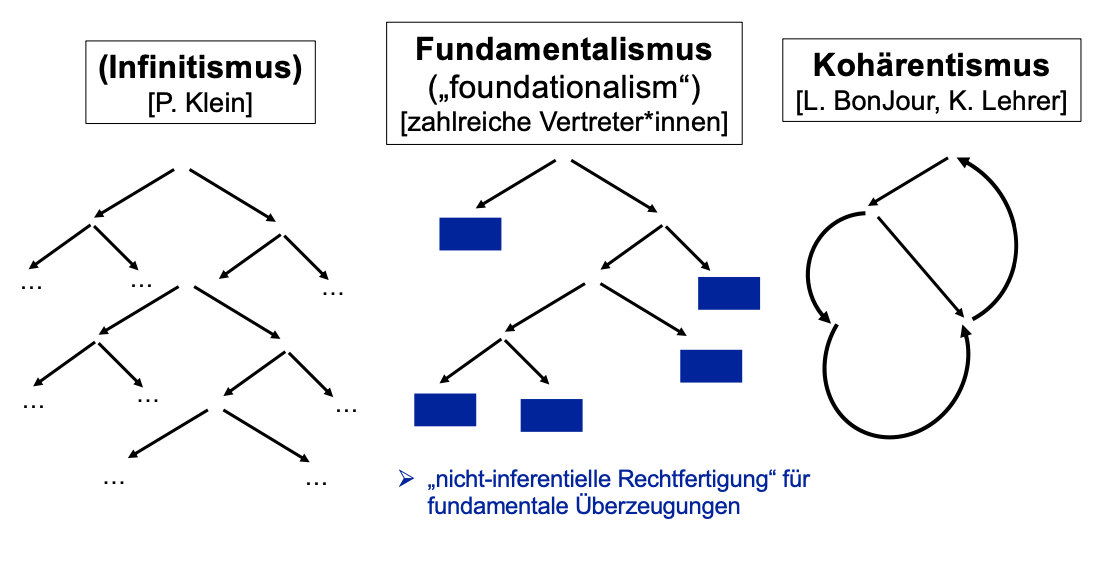
\includegraphics[height=6cm]{images/argumentationsketten.png}\endcenter}

\subsubsection{Argument des nicht-feststellbaren skeptischen Szenario}
Wir sprechen von nicht-feststellbaren skeptischen Szenarien, wenn wir dieses nicht von der Realität unterscheiden können und deren Schlussfolgerung ist, dass wir (fast) alle unsere alltäglichen Überzeugungen über die Aussenwelt aufgeben müssen. 

Bei Decartes ist dies das \textbf{Traumszenario} (Befinden wir uns in einem Traum?) oder das \textbf{Dämonszenario} (Ein bösartiges Wesen täuscht mir die Aussenwelt vor). Auch populär ist das zeitgenössische (Putnam) \textbf{Hirn-im-Tank-Szenario} (wir sind ein Gehirn im Tank und all unsere sensorischen Reize werden durch einen Computer simuliert).

\paragraph{Gehirn-im-Tank-Szenario} funktioniert so: (1) Wüsste ich, dass ich zwei Hände habe, dann weiss ich, dass ich kein Gehirn-im-Tank bin. Aber (2) ich weiss nicht, dass ich kein Gehirn-im-Tank bin! Also (\textit{modus tollens}) weiss ich nicht, ob ich Hände habe! Deswegen: Ich weiss nichts über die Aussenwelt.

\paragraph{Einwände}
\begin{enumerate}
	\item Mooreanismus von G. E. Moore (1873-1952) nach dem Motto <<Dein \textit{modus tollens} ist mein \textit{modus ponens}>> (wo du Rückschlüsse machst, mache ich Schlüsse vorwärts): (1) Wenn ich weiss, dass ich zwei Hände habe, dann weiss ich aiuch, dass ich kein GiT bin. (2) Ich weiss, dass ich zwei Hände habe! Also (3) bin ich kein GiT!

		Gemäss dem G. E. Moore müssen wir also ein deduktives Argument nicht akzeptieren, wenn wir seine Prämissen angreifen können. Das tut er im Mooreanismus, in welchem er Prämisse 2. des Gehirn-im-Tank Argumentes angreift. Damit muss er auch keine Skeptiker überzeugen können, sondern nur ihre Argumentation nicht akzeptieren. 
\end{enumerate}
\vspace{10pt}
{\centering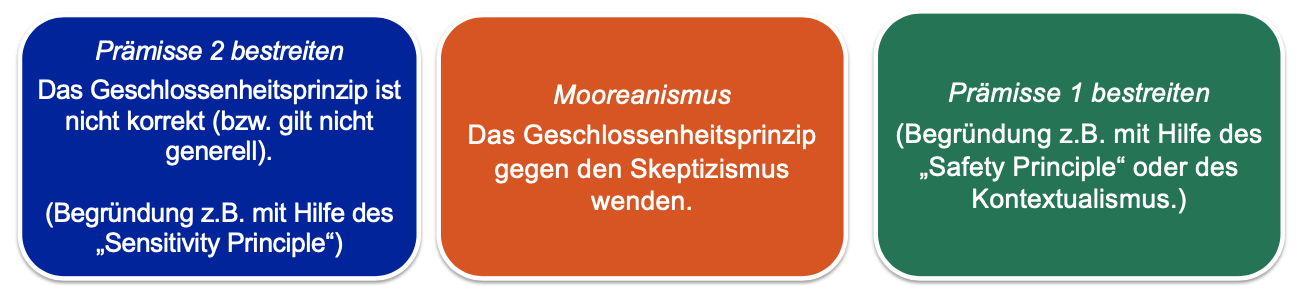
\includegraphics[width=\textwidth]{images/loesungsansaetze_gehirn_im_tank.png}\endcenter}


\section{Was ist Wissen?}
\paragraph{These (klassisches Analyze von Wissen)}
\begin{enumerate}
	\item Eine Person \textit{glaubt} an die Wahrheit des Sachverhalts
	\item Der Sachverhalt ist \textit{objektiv wahr}.
	\item Der Glaube an die Wahrheit des Sachverhalts ist durch die Person \textit{gerechtfertigt / gut begründet}
\end{enumerate}

\subsection{Das Gettier-Problem}
Das Problem wurde von Edmund Gettier (1927-2021) vorgeschlagen und seitdem intensiv diskutiert. Diese Fälle widersprechen der klassischen Analyse von Wissen:
\subsubsection{1. Gettier Fall}
\begin{enumerate}
	\item Smith hat gute Gründe anzunehmen, dass sein Konkurrent den Job erhalten wird und zusätzlich Geld in der Tasche hat. 
	\item Smith schliesst logisch aus 1. darauf, dass der Mann den Job erhalten wird, der Geld in der Tasche hat. 
	\item Smith erhält jedoch den Job und hat, ohne es zu ahnen, selber Geld in der Tasche. 
\end{enumerate}

Man kann also sagen, dass Smith eine gerechtfertigte Überzeugung hat, wer den Job erhält, ohne es effektiv zu wissen! Wir können schlussfolgern, dass eine gerechtfertigte Überzeugung \textbf{nicht hinreichend für Wissen} ist und daraus ergibt sich, dass die klassische Analyse von Wissen falsch ist. 

\subsubsection{2. Gettier Fall}
\begin{enumerate}
	\item Bertie hat gute Gründe dafür, dass ihre Uhr zuverlässig funktioniert (immer gewartete und qualitative Uhr)
	\item Berties sieht auf die Uhr und erkennt, dass 12:00 ist.
	\item Aber die Uhr ist vor 12:00 stehen geblieben!
\end{enumerate}
Man kann also sagen, dass Bertie eine gerechtfertigte Überzeugung hat, was für Uhrzeit gerade ist, ohne es effektiv zu wissen! Wir können schlussfolgern, dass eine gerechtfertigte Überzeugung \textbf{nicht hinreichend für Wissen} ist und daraus ergibt sich, dass die klassische Analyse von Wissen falsch ist. 

\section{Rechtfertigungen und Überzeugungen}
Eine Überzeugung ist gerechtfertigt, gdw. sie gute begründet ist. Traditionell wird angenommen, dass diese Gründe \textit{mentale Zustände} sind (\textbf{Mentalismus}).


\subsection{Internalismus}
Der Internalismus geht davon aus, dass das, was Überzeugungen gerechtfertigt macht, im wesentlichen von der Person selber ausgeht. Somit ist man für diese verantwortlich. 

\subsubsection{Mentalismus (Subjektivismus) als epistemischer Internalismus}
Eine Überzeugung ist gerechtfertigt, gdw. jemand mentale Zustände (andere Überzeugungen und Sinneseindrücke) hat, die dafür gute Gründe liefern.
\paragraph{Abgrenzung} Wer den Mentalismus akzeptiert, der akzeptiert auch den Zugangsinternalismus. Denn es ist plausibel, dass die Überzeugungen, die etwas rechtfertigen, auch mental zugänglich sind. 

\subsubsection{Zugangsinternalismus als epistemischer Internalismus}
Eine Überzeugung ist gerechtfertigt, gdw. gute Gründe hat, die jemand kognitiv zugänglich sind. 
\paragraph{Abgrenzung} Wer den Zugangsinternalismus akzeptiert, der muss nicht zwingend den Mentalismus akzeptieren, da auch nicht-mentale Zustände, die dem Subjekt kognitiv bekannt sind, dessen Überzeugungen rechtfertigen können. 

\subsection{Externalismus}
Der Externalismus ist zunächst eine Negation des Internalismus. 
\subsubsection{Non-Mentalismus (Objektivismus) als epistemischer Externalismus}
\paragraph{These} (Im Vergleich mit Mentalismus) Gerechtfertigte Überzeugungen können auch auf nicht-mentalen Umstände/Tatsachen begründet sein. 

\subsubsection{Zugangsexternalismus als epistemischer Externalismus}
Die Gründe, die Überzeugungen rechtfertigen, könne auch Umstände sein, die nicht kognitiv bekannt sind. 

\subsection{Zugangsexternalistischer Reliabilismus (Prozessreliabilismus)}
\paragraph{These} Eine Überzeugung ist gerechtfertigt, gdw. sie das Resultat eines zuverlässigen Prozesses ist, also eine Prozesses, der mit (de facto) hoher Wahrscheinlichkeit wahre Überzeugungen hervorbringt. 
\paragraph{Erklärung} Vertreten durch Alvin Goldman, besagt der Reliabilismus, dass gerechtfertige Überzeugungen aus Prozessen resultiert, die zuverlässig sind. Zum Beispiel die visuelle Wahrnehmung (wenn funktional), das Nachlesen in vertrauenswürdigen Quellen, die mathematische Beweisführung, etc. 

Der Reliabilismus ist Teil der zugangsexternalistischen Theorien, da die Zuverlässigkeit eines Prozesses (meist) nicht kognitiv zugänglich ist. 

Begründet auf diesen Ansichten, bildet sich die \textbf{reliabilistische Analyse des Wissens}. Eine Person weiss, dass etwas wahr ist, gdw. 
\begin{enumerate}
	\item sie glaubt, dass es wahr ist (hat die Überzeugung),
	\item es auch wirklich wahr ist
	\item und die Überzeugung Produkt eines zuverlässigen Prozesses ist. 
\end{enumerate}

\paragraph{Antworten auf Probleme}
\begin{enumerate}
	\item Agrippas Trilemma (klassischer Skeptizismus): Der Relliabilist antwortet auf das Trilemma, das besagt, dass alle Überzeugungen auf andere Überzeugungen gestützt sein müssen, damit, dass Überzeugungen als Produkt des zuverlässigen Prozesses nicht auf weitere Überzeugungen gestützt sein müssen. 
	\item Nicht-feststellbare skeptische Szenario: Der Reliabilist hilft der mooreanischen Strategie; Ein zuverlässiger Prozess (interozeptiven und exterozeptiven Wahrnehmung) resultiert darin, dass ich zwei Hände habe. Deswegen funktioniert das umgekehrte mooreanische Argument.
	\item Gettier-Probleme: Die <<gerechtfertigten>> Überzeugung in den Gettier-Fällen sind nicht Resultat eines zuverlässigen Prozesses (aber in hohem Mass rational), weswegen diese kein Wissen darstellen. Aber lassen sich alle Gettier-Fälle so abwehren?
\end{enumerate}

\subsection{Nozicks zugangsexternalistische Sensitivitätstheorie}
\paragraph{These} Man weiss, dass etwas wahr ist, gdw.
\begin{enumerate}
	\item man glaubt, dass etwas wahr ist (hat die Überzeugung),
	\item es effektiv wahr ist
	\item und wenn es falsch wäre, dann würde man es nicht glauben, dass es wahr wäre (für die Wahrheit sensitive Überzeugung).
\end{enumerate}
\paragraph{Erklärung} Die Theorie baut auf der Sensitivitätsbedingung auf. Da diese nicht kognitiv zugänglich sein muss, ist dies eine Theorie des Zugangsexternalismus. 

Die Argumentation, auf den ersten Blick banal, auf den zweiten verwirrend, funktioniert folgendermassen: Für jede Proposition wird analysiert, ob wir das gleiche auch denken würden, wäre es nicht wahr. So kann ich sagen, dass ich die Prüfung bestanden habe und es handelt sich um Wissen (vorausgesetzt, es ist wahr und ich glaube daran), genau dann, wenn ich sagen würde, dass ich sie nicht bestanden hätte, hätte ich sie nicht bestanden. Wissen wird also durch den Umkehrschluss definiert. 
\paragraph{Antworten auf Probleme}
\begin{enumerate}
	\item Nicht-feststellbares skeptisches Szenario: Nozick bestreitet die Prämisse 1., die besagt, dass, wenn man weiss, dass man zwei Hände hat, kein Gehirn-Im-Tank sein kann. Laut ihm kann man wissen, dass man zwei Hände hat und gleichzeitig (Prämisse 2) nicht wissen, dass man kein Gehirn im Tank ist. Somit bestreitet er das Geschlossenheitsprinzip!
	\item Gettier-Problem: Nozick betrachtet den zweiten Gettier Fall und antwortet darauf, dass kein Wissen vorliegt, denn wäre es nicht 12:00 Uhr, würde die Person trotzdem glauben, dass es 12:00 Uhr ist. 
\end{enumerate}

\section{Das Problem des Wertes des Wissens}
Der Konflikt um den Wert des Wissens, lässt sich folgendermassen illustrieren: Macht es effektiv einen Unterschied, ob jemand zufällig den richtigen und schnellsten Weg zum Bahnhof einschlägt, oder ob er diesen kennt, aber beide Parteien den gleichen Weg einschlagen (gleicher praktischer Nutzen)? Oder anders ausgedrückt, in Bezug auf den Reliabilismus: Macht es einen Unterschied, ob eine wahre Überzeugung Resultat eines zuverlässigen Prozesses ist oder einfach so geformt wurde?

{\centering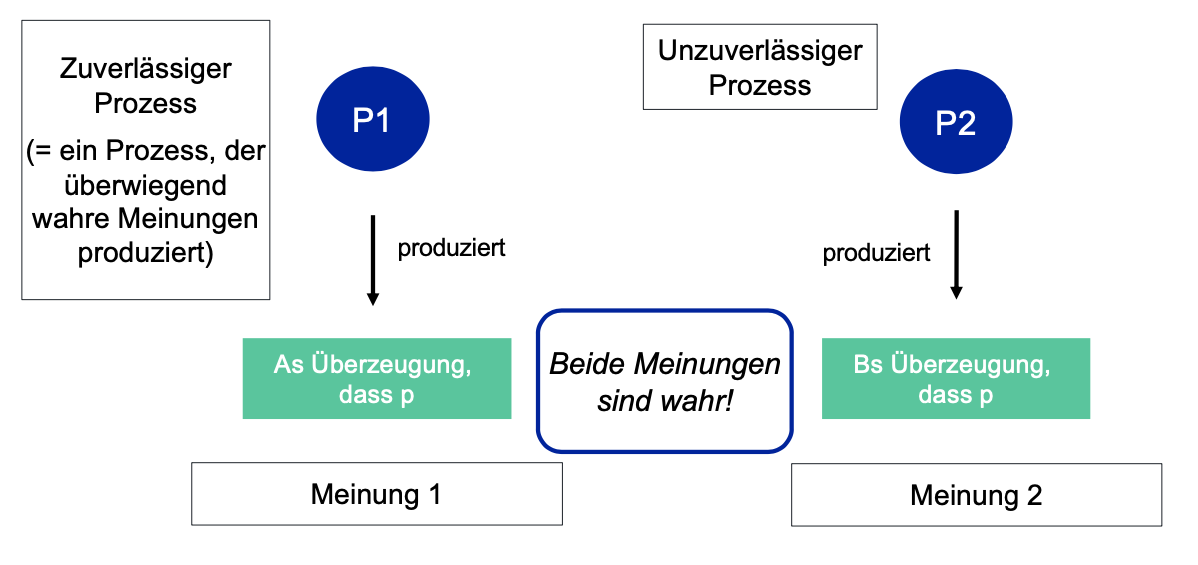
\includegraphics[height=6cm]{images/wahre_ueberzeugungen_und_zufaellige_ueberzeugungen.png}\endcenter}

\textbf{Schlussfolgerung}: Abgesehen von der Zuverlässigkeit bei einer Wiederholung des Experimentes, lässt sich sagen, dass es keine Unterscheidung zwischen zwei Überzeugungen gibt, abhängig davon, wie sie kreiert wurden (ob durch einen zuverlässigen Prozess oder durch Zufall).

\end{document}